%
% $RCSfile: knowledge_management_system.tex,v $
%
% Copyright (C) 2002-2008. Christian Heller.
%
% Permission is granted to copy, distribute and/or modify this document
% under the terms of the GNU Free Documentation License, Version 1.1 or
% any later version published by the Free Software Foundation; with no
% Invariant Sections, with no Front-Cover Texts and with no Back-Cover
% Texts. A copy of the license is included in the section entitled
% "GNU Free Documentation License".
%
% http://www.cybop.net
% - Cybernetics Oriented Programming -
%
% http://www.resmedicinae.org
% - Information in Medicine -
%
% Version: $Revision: 1.1 $ $Date: 2008-08-19 20:41:07 $ $Author: christian $
% Authors: Christian Heller <christian.heller@tuxtax.de>
%

\section{Knowledge Management System}
\label{knowledge_management_system_heading}
\index{Knowledge Management System}

Section \ref{virtual_and_real_world_heading} justified a separation of knowledge
from system control software. Section \ref{system_and_knowledge_heading}
considered the effects of that separation to traditional software design. What
remains to be investigated is how a system adhering to a separation of that
kind would have to look like.

%
% $RCSfile: hardware_connection.tex,v $
%
% Copyright (C) 2002-2008. Christian Heller.
%
% Permission is granted to copy, distribute and/or modify this document
% under the terms of the GNU Free Documentation License, Version 1.1 or
% any later version published by the Free Software Foundation; with no
% Invariant Sections, with no Front-Cover Texts and with no Back-Cover
% Texts. A copy of the license is included in the section entitled
% "GNU Free Documentation License".
%
% http://www.cybop.net
% - Cybernetics Oriented Programming -
%
% http://www.resmedicinae.org
% - Information in Medicine -
%
% Version: $Revision: 1.1 $ $Date: 2008-08-19 20:41:07 $ $Author: christian $
% Authors: Christian Heller <christian.heller@tuxtax.de>
%

\subsection{Hardware Connection}
\label{hardware_connection_heading}
\index{Knowledge-Hardware Connection}
\index{Operating System}
\index{OS}
\index{Daemon}
\index{Knowledge}
\index{Control Software}
\index{Hardware}

Knowledge is \emph{passive}. What makes use of knowledge is the \emph{active}
parts of a system, in the case of computers a process like the
\emph{Operating System} (OS) or applications using external configuration
settings. They are able to both, communicate with hardware and adopt knowledge,
for it to be memorised and processed.

Traditionally, OS make use of a number of helper processes (\emph{Daemons},
section \ref{local_process_heading}), for services like printing or email
delivery, which may also be used by applications. This work, however, wants to
unify services in just one low-level system control process. Another issue are
the varying communication paradigms a classical application has to consider.
Persistence mechanisms, user interfaces, remote communication -- they all have
their specific requirements, whether supported by a special framework (section
\ref{framework_heading}) or not. This work wants to simplify communication in a
way that applications do not have to do more than issuing a simple \emph{send}
or \emph{receive} instruction, adding the desired language of communication. By
disburdening applications from low-level communication and signal (event)
handling responsibilities, they become purely passive knowledge (statics) which
cannot act itself, but needs to be read and interpreted by an active control
process (dynamics).

\begin{figure}[ht]
    \begin{center}
        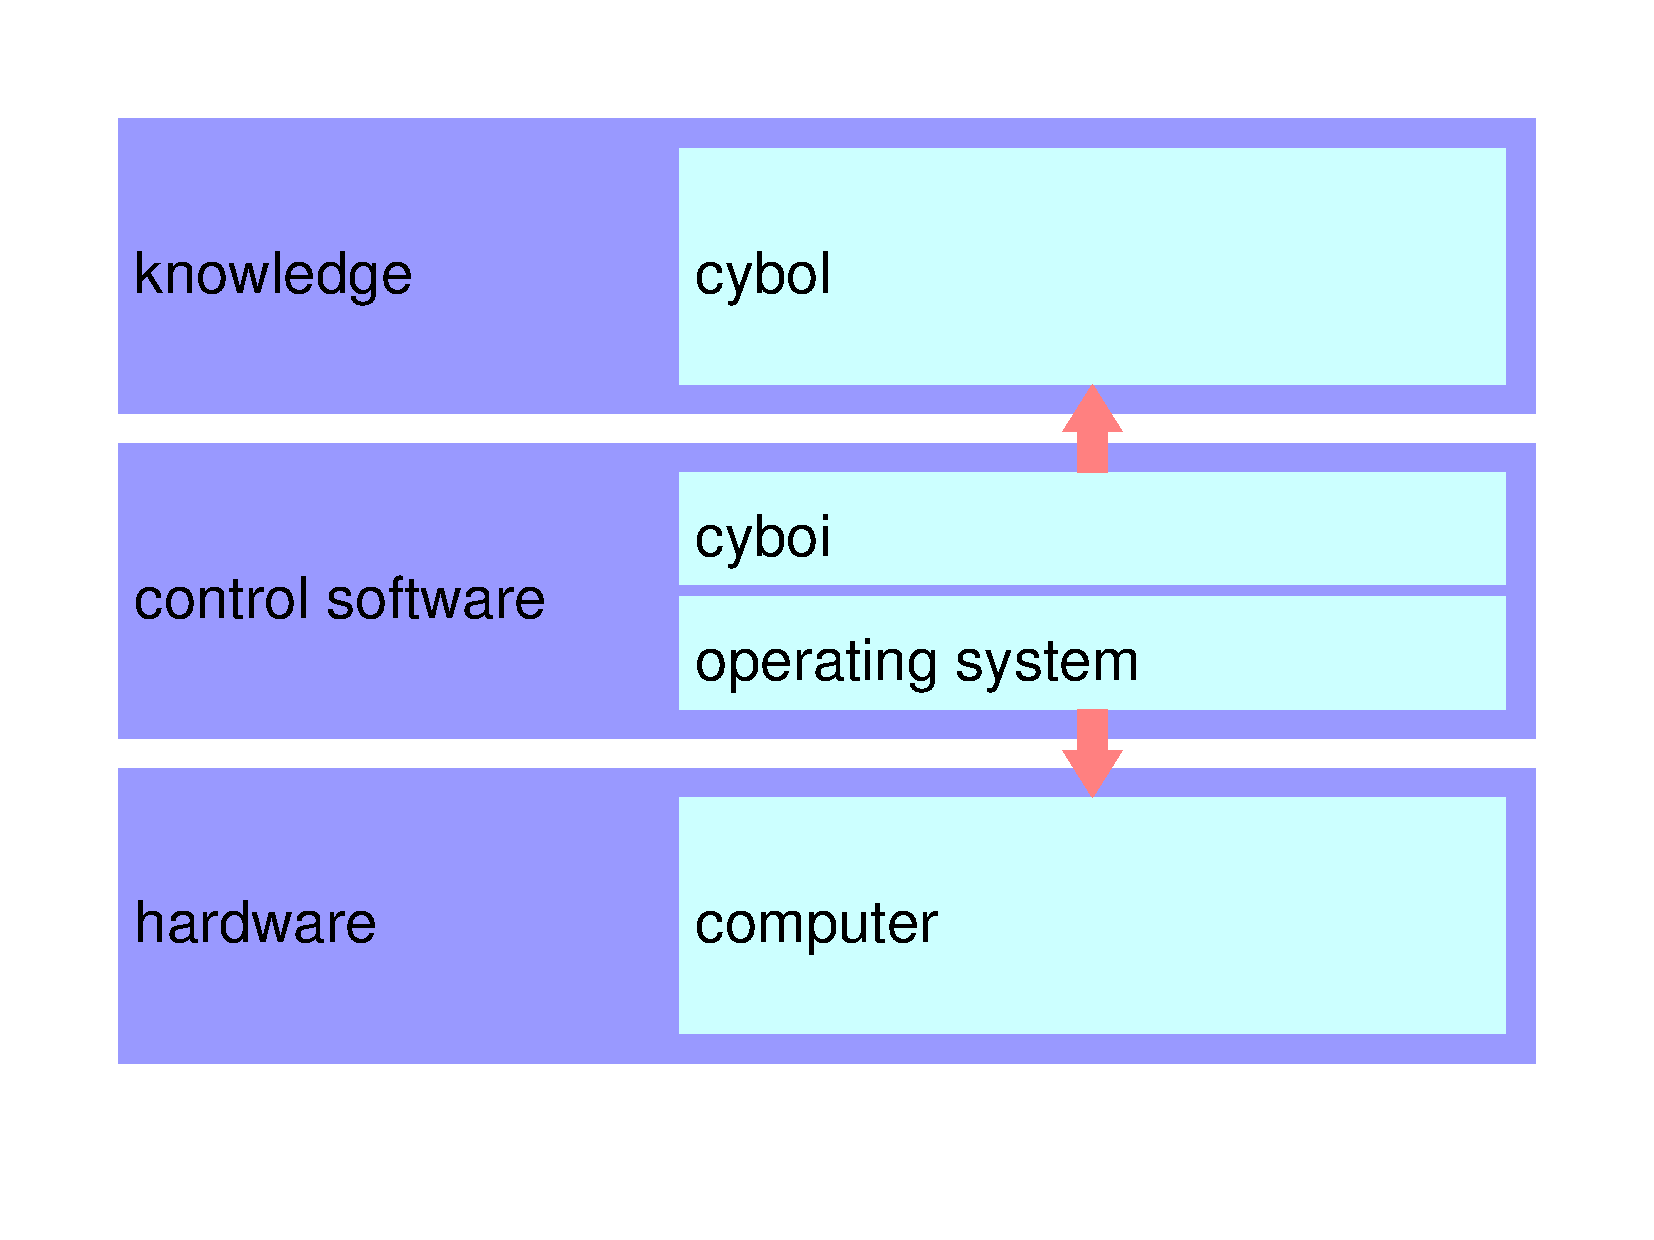
\includegraphics[scale=0.3,angle=-90]{graphic/connection.pdf}
        \caption{Knowledge -- Hardware Connection}
        \label{connection_figure}
    \end{center}
\end{figure}

Three main layers of information crystallise out: \emph{Knowledge},
\emph{Control Software} and \emph{Hardware} (figure \ref{connection_figure}).
Tanenbaum \cite{tanenbaum1999} calls the latter two \textit{logically equivalent}
(section \ref{paradigm_and_language_heading}), because one could replace the
other. It is indeed up to the computer designer to decide how much control
software should get burned into hardware. Hence, the important separation is
between \emph{Knowledge} on one side and \emph{Hardware} together with
\emph{Control Software} on the other.

The previous sections \ref{mind_and_body_heading}, \ref{brain_regions_heading}
and \ref{cell_division_heading} tried to justify this separation by looking at
nature. Knowledge is the equivalent of: \emph{Mind} (philosophically) and the
virtual information stored in a human brain's \emph{Hippocampus} and
\emph{Cerebral Cortex}, as well as of the information encoded in a biological
cell's \emph{Desoxy Ribo Nucleic Acid} (DNA). Hardware and control software are
the equivalent of: (philosophically) \emph{Body}, (neurologically) parts of the
human brain (\emph{Midbrain}, \emph{Basal Ganglia}) which coordinate the input/
output (i/o) of knowledge and (biologically) \emph{Ribo Nucleic Acid} (RNA)
molecules transmitting the genetic information from the DNA into proteins.

Chapters \ref{cybernetics_oriented_language_heading} and
\ref{cybernetics_oriented_interpreter_heading} will describe the
\emph{Cybernetics Oriented Language} (CYBOL) as knowledge specification format
and the \emph{Cybernetics Oriented Interpreter} (CYBOI) as system being able to
handle such knowledge, as well as to serve as hardware interface. All
hardware-controlling functionality needs to be present within either CYBOI or
the underlying \emph{Operating System} (OS) closely coupled with it. Together,
they are the active entity allowing virtual and real world (knowledge and
hardware) to communicate.

The remaining sections of this chapter describe important elements belonging to
a control software's architecture. More detailed descriptions of the
architecture and functionality will be given in chapter
\ref{cybernetics_oriented_interpreter_heading} devoted to CYBOI only.

%
% $RCSfile: memory.tex,v $
%
% Copyright (C) 2002-2008. Christian Heller.
%
% Permission is granted to copy, distribute and/or modify this document
% under the terms of the GNU Free Documentation License, Version 1.1 or
% any later version published by the Free Software Foundation; with no
% Invariant Sections, with no Front-Cover Texts and with no Back-Cover
% Texts. A copy of the license is included in the section entitled
% "GNU Free Documentation License".
%
% http://www.cybop.net
% - Cybernetics Oriented Programming -
%
% http://www.resmedicinae.org
% - Information in Medicine -
%
% Version: $Revision: 1.1 $ $Date: 2008-08-19 20:41:07 $ $Author: christian $
% Authors: Christian Heller <christian.heller@tuxtax.de>
%

\subsection{Memory}
\label{memory_heading}
\index{Memory}
\index{Persistent Memory}
\index{Transient Memory}
\index{Volatile Memory}
\index{Sensory Memory}
\index{Long Term Memory}
\index{LTM}
\index{Short Term Memory}
\index{STM}
\index{Knowledge Memory}
\index{Signal Memory}
\index{Internal Memory}
\index{Input/ Output Memory}
\index{Event Queue}

The application/ domain knowledge a control software processes resides in a
\emph{Memory}. Two different kinds known from \emph{Informatics} are the
\emph{persistent} and \emph{transient} (\emph{volatile}) memory (section
\ref{persistent_and_transient_heading}). For the system architecture
investigated in this section, the term \emph{Memory} does not refer to
hardware, but to a special data structure for knowledge storage.

Section \ref{short_and_long_term_memory_heading} introduced the
\emph{Sensory Memory}, \emph{Long Term Memory} (LTM) and \emph{Short Term Memory}
(STM), so labelled by the science of psychology. Sensory memory stores data
arriving from input organs; LTM stores past contents; STM holds temporary
information to be processed within the system. A knowledge-processing system
with human archetype -- such as the one proposed in this work -- needs to have
equivalents for all three of them. Figure \ref{system_figure} illustrates a
system based on four kinds of memory:

\begin{itemize}
    \item[-] Knowledge Memory (equivalent of LTM)
    \item[-] Signal Memory (equivalent of STM)
    \item[-] Internal Memory (program-internal data)
    \item[-] Input/ Output Memories (sensory data)
\end{itemize}

The \emph{Knowledge Memory} is represented by one single root node that is able
to keep knowledge hierarchies of arbitrary size. The \emph{Signal Memory} is
much the same as the \emph{Event Queue} in classical systems.
\emph{Internal Memory} and \emph{Input/ Output Memories} are helper memories
for storing system-internal parameters.

\begin{figure}[ht]
    \begin{center}
        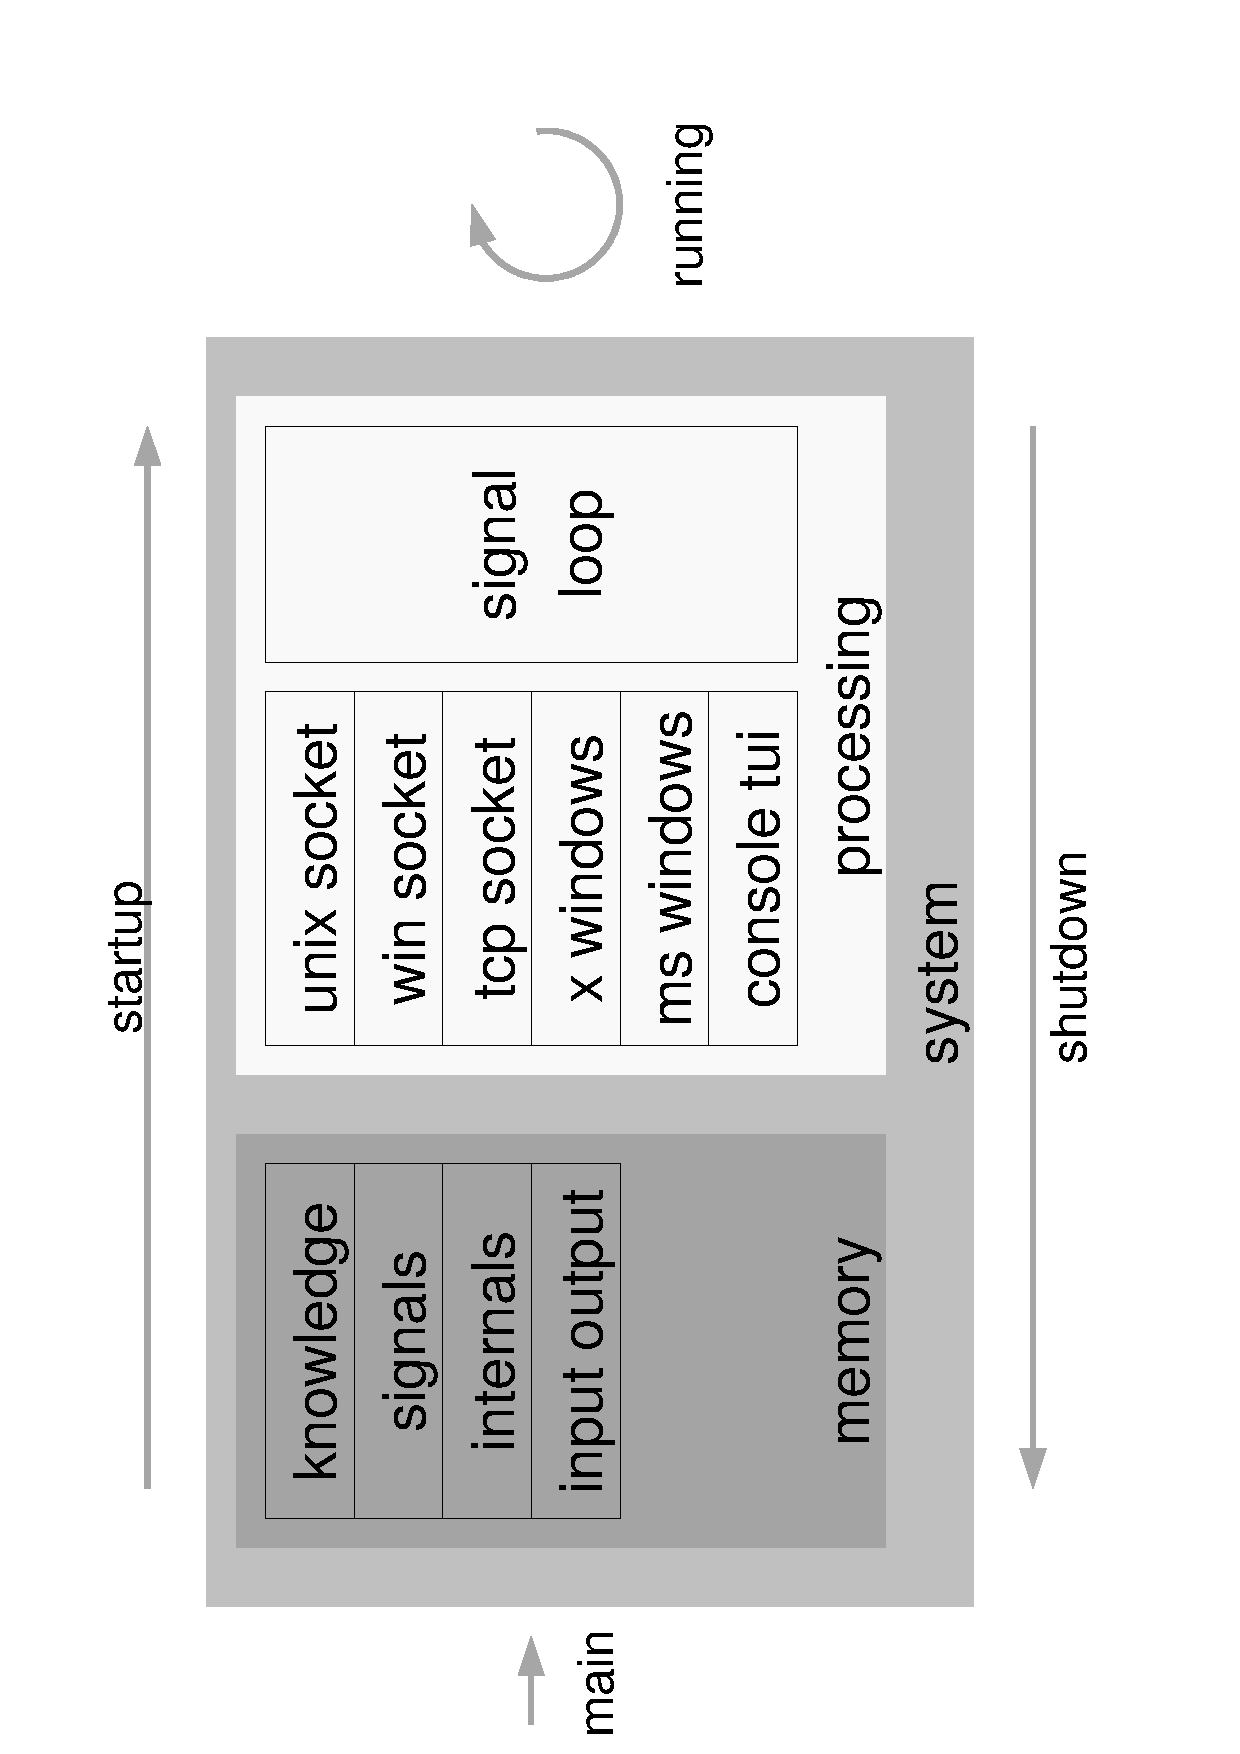
\includegraphics[scale=0.3,angle=-90]{graphic/system.pdf}
        \caption{System with Memory Structures, Processing Loops and Lifecycle}
        \label{system_figure}
    \end{center}
\end{figure}

%
% $RCSfile: processing.tex,v $
%
% Copyright (C) 2002-2008. Christian Heller.
%
% Permission is granted to copy, distribute and/or modify this document
% under the terms of the GNU Free Documentation License, Version 1.1 or
% any later version published by the Free Software Foundation; with no
% Invariant Sections, with no Front-Cover Texts and with no Back-Cover
% Texts. A copy of the license is included in the section entitled
% "GNU Free Documentation License".
%
% http://www.cybop.net
% - Cybernetics Oriented Programming -
%
% http://www.resmedicinae.org
% - Information in Medicine -
%
% Version: $Revision: 1.1 $ $Date: 2008-08-19 20:41:08 $ $Author: christian $
% Authors: Christian Heller <christian.heller@tuxtax.de>
%

\subsection{Processing}
\label{processing_heading}
\index{Processing of Knowledge}
\index{Signal}
\index{Event}
\index{Signal Memory}
\index{Event Queue}
\index{Signal Loop}
\index{Waiting Loop}
\index{Priority of a Signal}
\index{Prioritising}
\index{Operating System}
\index{OS}
\index{Intra System Communication}
\index{Inter System Communication}
\index{Message}

While knowledge as such is static at a given time instant, its \emph{Processing}
and manipulation over time are dynamic. The processing is triggered by some
\emph{Signal} (also called \emph{Event}), which is a state change known to the
system. Such \textit{signs with defined meaning}, as the Duden Encyclopedia
\cite{duden} calls them, can be most different in their appearance and
communication channel used.

Signals are commonly stored in a \emph{Signal Memory} (also called
\emph{Event Queue}), as mentioned in the previous section. An endlessly running
\emph{Signal Loop} (also called \emph{Waiting Loop}) as illustrated in figure
\ref{system_figure} is constantly checking the signal memory for new signals.
Once a signal is detected, it gets removed from the signal memory and handled
by the system. The signal with highest \emph{Priority} is processed first. The
later chapter \ref{cybernetics_oriented_interpreter_heading} will explain
further details and deliver a more functional illustration (figure
\ref{dependencies_figure}).

Section \ref{brain_regions_heading} mentioned the \emph{Hypothalamus} and
\emph{Limbic System} as parts of the human brain producing emotions. Section
\ref{information_processing_model_heading} wrote that the processing of a signal
may be greatly influenced by the meaningfulness or \emph{Emotional Content} of
an item. Well, software systems do not work with emotions, but signals can be
assigned a \emph{Priority}, which is somewhat comparable. \emph{Prioritising}
as technique stems from \emph{Operating System} (OS) research and can be well
applied in the described knowledge-processing system: Signals can be filtered
in a way that unimportant signals get discarded; urgent signals get processed
right away; less important but meaningful signals get queued for later handling.

All \emph{intra-system} and \emph{inter-system} communication is based on the
exchange of knowledge via signals. A signal can transport simple or more complex
\emph{Messages}, mostly in encoded form. The communication details, including
encoding and decoding procedures for knowledge model translation, and the logic
after which an input state gets transferred into an output state are the topic
of chapter \ref{state_and_logic_heading}.

Besides the \emph{declarative} \emph{Long Term Memory} (LTM), section
\ref{short_and_long_term_memory_heading} mentioned the \emph{procedural}
(non-declarative) LTM, enabling humans to carry out a \emph{Background Task},
without having to consciously control it. A similar principle is applied for
input/ output (i/o) handling, in the described knowledge processing system.
Independent \emph{Threads} running their own loops control a special i/o
mechanism (like \emph{UNIX socket etc.}), each (figure \ref{system_figure}).

\section{An Extended Component Lifecycle}

The CYBOP lifecycle of components is an extension of the lifecycle idea of Apache
-- basically the same idea but another background and realization.\\
All \emph{whole-part associations} between objects were organized
under the rules of the component lifecycle. Analogous to the
lifecycle of organic cells, the relations were created and
destroyed in a sequence of lifecycle steps. These steps are
realized as method calls on the components (see figure \ref{State
Diagram of CYBOB's Component Lifecycle}).
\includepicture{8}{eps/lebenszyklusEng.eps}{State Diagram of CYBOB's Component Lifecycle}{State Diagram of CYBOB's Component Lifecycle}{State Diagram of CYBOB's Component Lifecycle} {State Diagram of CYBOB's Component Lifecycle}

%\input{instantiation} (clone, serialisation, knowledge template and -instance)
%\input{template_and_model} (activate when replication/ cloning is activated, too
% = persistent knowledge template versus transient knowledge model
